% Titel: Ziel des Versuchs
% Theorie: Physikalische Grundlagen von Versuch/Messverfahren, Gleichungen ohne Herleitung knapp erklären
\section{Theorie}
\label{sec:theorie}

Im abgeschlossenen System fließt Wärme immer vom wärmeren zum kälteren Reservoir. Dieser Wärmefluss
ist jedoch umkehrbar, indem äußere Energie zugeführt wird. Realisieren lässt sich dieser Prozess in
der Wärmepumpe durch das Aufwenden mechanischer Arbeit.

\begin{figure}
	\centering
	\vspace{1.23ex}
	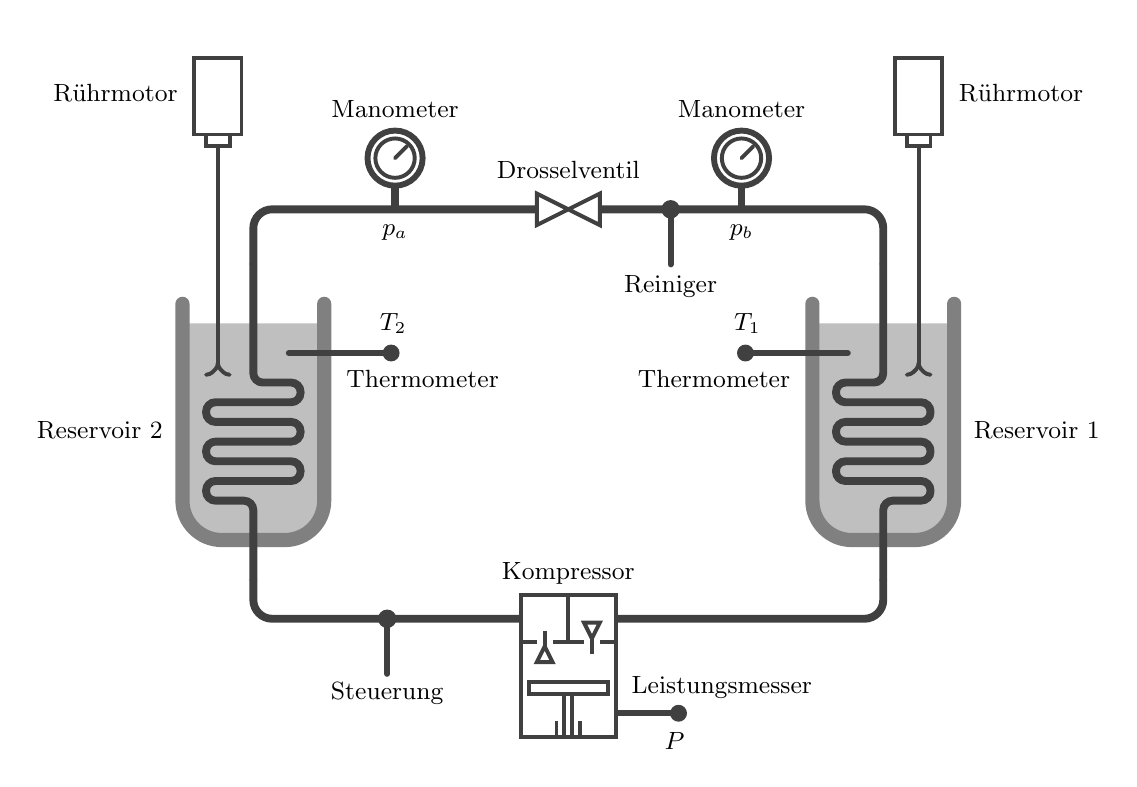
\begin{tikzpicture}
		\tikzstyle{every node} = [font = \small]

% frame
\draw[draw=white] 
	(0,0) -- ++(0,9) -- ++(8,0) -- ++(0,-9) -- cycle;

% valve
\draw[draw=darkgray, line width=0.5mm] 
	(3.6,6.7) -- ++(0,-0.2) -- ++(0.8,0.4) -- ++(0,-0.4) -- ++(-0.8,0.4) -- cycle;

% compresser
\draw[draw=darkgray, line width=0.5mm] 
	(3.4,0) -- ++(0,1.8) -- ++(1.2,0) -- ++(0,-1.8) -- cycle;
\draw[draw=darkgray, line width=0.5mm] 
	(4,1.8) -- ++(0,-0.6);
\draw[draw=darkgray, line width=0.5mm] 
	(3.8,1.2) -- ++(0.4,0);
\draw[draw=darkgray, line width=0.5mm] 
	(3.4,1.2) -- ++(0.2,0);
\draw[draw=darkgray, line width=0.5mm] 
	(4.6,1.2) -- ++(-0.2,0);
\draw[draw=darkgray, line width=0.5mm] 
	(3.7,1.35) -- ++(0,-0.2);
\draw[draw=darkgray, line width=0.5mm] 
	(3.7,1.15) -- ++(-0.1,-0.2) -- ++(0.2,0) -- cycle;
\draw[draw=darkgray, line width=0.5mm] 
	(4.3,1.25) -- ++(0,-0.2);
\draw[draw=darkgray, line width=0.5mm] 
	(4.3,1.25) -- ++(-0.1,0.2) -- ++(0.2,0) -- cycle;
\draw[draw=darkgray, line width=0.5mm] 
	(3.5,0.7) -- ++(1,0) -- ++(0,-0.15) -- ++(-1,0) -- cycle;
\draw[draw=darkgray, line width=0.5mm] 
	(3.95,0.55) -- ++(0,-0.55);
\draw[draw=darkgray, line width=0.5mm] 
	(4.05,0.55) -- ++(0,-0.55);
\draw[draw=darkgray, line width=0.5mm] 
	(3.85,0.2) -- ++(0,-0.2);
\draw[draw=darkgray, line width=0.5mm] 
	(4.15,0.2) -- ++(0,-0.2);

% wattmeter
\draw[draw=darkgray, line width=0.75mm] 
	(4.6,0.3) -- (5.4,0.3);
\draw[draw=darkgray, fill=darkgray] 
	(5.4,0.3) circle (1mm);

% control
\draw[draw=darkgray, line width=0.75mm, line cap=round] 
	(1.7,1.5) -- (1.7,0.8);
\draw[draw=darkgray, fill=darkgray] 
	(1.7,1.5) circle (1.1mm);

% diffuser
\draw[draw=darkgray, line width=0.75mm, line cap=round] 
	(5.3,6.7) -- (5.3,6);
\draw[draw=darkgray, fill=darkgray] 
	(5.3,6.7) circle (1.1mm);

% left

% bucket
\draw[draw=lightgray, fill=lightgray, line width=0mm, line cap=round, rounded corners=5mm] 
	(-0.9,5.25) -- ++(0,-2.75) -- ++(1.8,0) -- ++(0,2.75);
\draw[draw=gray, line width=1.8mm, line cap=round, rounded corners=5mm] 
	(-0.9,5.5) -- ++(0,-3) -- ++(1.8,0) -- ++(0,3);
% mixer
\draw[draw=darkgray, line width=0.5mm] 
	(-0.45,7.5) -- ++(0,-2.75);
\draw[draw=darkgray, line width=0.5mm, line cap=round, rounded corners=0.45mm] 
	(-0.45,4.75) -- ++(0,-0.05) -- ++(-0.1,-0.1) -- ++(-0.05,0);
\draw[draw=darkgray, line width=0.5mm, line cap=round, rounded corners=0.45mm] 
	(-0.45,4.75) -- ++(0,-0.05) -- ++(0.1,-0.1) -- ++(0.05,0);
\draw[draw=darkgray, line width=0.5mm] 
	(-0.6,7.65) -- ++(0,-0.15) -- ++(0.3,0) -- ++(0,0.15);
\draw[draw=darkgray, line width=0.5mm] 
	(-0.75,7.65) -- ++(0.6,0) -- ++(0,0.975) -- ++(-0.6,0) -- cycle;
% thermometer
\draw[draw=darkgray, line width=0.75mm, line cap=round] 
	(0.45,4.875) -- (1.75,4.875);
\draw[draw=darkgray, fill=darkgray] 
	(1.75,4.875) circle (1mm);
% manometer
\draw[draw=darkgray, line width=1mm] 
	(1.8,6.7) -- (1.8,7);
\draw[draw=darkgray, line width=0.75mm] 
	(1.8,7.35) circle (3.5mm);
\draw[draw=darkgray, line width=0.5mm] 
	(1.8,7.35) circle (2.5mm);
\draw[draw=darkgray, line width=0.5mm, line cap=round] 
	(1.8,7.35) -- ++(0.15,0.15);
% snake
\draw[draw=darkgray, line width=1mm, line cap=round, rounded corners=1.2mm] 
	(0,6) -- ++(0,-1.5) -- ++(0.6,0) -- ++(0,-0.25) -- ++(-1.2,0) -- ++(0,-0.25)
	-- ++(1.2,0) -- ++(0,-0.25) -- ++(-1.2,0) -- ++(0,-0.25)
	-- ++(1.2,0) -- ++(0,-0.25) -- ++(-1.2,0) -- ++(0,-0.25)
	-- ++(0.6,0) -- (0,2);
\draw[draw=darkgray, line width=1mm, rounded corners=2.4mm] 
	(0,2) -- (0,1.5) -- (3.4,1.5);
\draw[draw=darkgray, line width=1mm, rounded corners=2.4mm] 
	(0,6) -- (0,6.7) -- (3.6,6.7);

% right

% bucket
\draw[draw=lightgray, fill=lightgray, line width=0mm, line cap=round, rounded corners=5mm] 
	(7.1,5.25) -- ++(0,-2.75) -- ++(1.8,0) -- ++(0,2.75);
\draw[draw=gray, line width=1.8mm, line cap=round, rounded corners=5mm] 
	(7.1,5.5) -- ++(0,-3) -- ++(1.8,0) -- ++(0,3);
% mixer
\draw[draw=darkgray, line width=0.5mm] 
	(8.45,7.5) -- ++(0,-2.75);
\draw[draw=darkgray, line width=0.5mm, line cap=round, rounded corners=0.45mm] 
	(8.45,4.75) -- ++(0,-0.05) -- ++(-0.1,-0.1) -- ++(-0.05,0);
\draw[draw=darkgray, line width=0.5mm, line cap=round, rounded corners=0.45mm] 
	(8.45,4.75) -- ++(0,-0.05) -- ++(0.1,-0.1) -- ++(0.05,0);
\draw[draw=darkgray, line width=0.5mm] 
	(8.3,7.65) -- ++(0,-0.15) -- ++(0.3,0) -- ++(0,0.15);
\draw[draw=darkgray, line width=0.5mm] 
	(8.15,7.65) -- ++(0.6,0) -- ++(0,0.975) -- ++(-0.6,0) -- cycle;
% thermometer
\draw[draw=darkgray, line width=0.75mm, line cap=round] 
	(7.55,4.875) -- (6.25,4.875);
\draw[draw=darkgray, fill=darkgray] 
	(6.25,4.875) circle (1mm);
% manometer
\draw[draw=darkgray, line width=1mm] 
	(6.2,6.7) -- (6.2,7);
\draw[draw=darkgray, line width=0.75mm] 
	(6.2,7.35) circle (3.5mm);
\draw[draw=darkgray, line width=0.5mm] 
	(6.2,7.35) circle (2.5mm);
\draw[draw=darkgray, line width=0.5mm, line cap=round] 
	(6.2,7.35) -- ++(0.15,0.15);
% snake
\draw[draw=darkgray, line width=1mm, line cap=round, rounded corners=1.2mm] 
	(8,6) -- ++(0,-1.5) -- ++(-0.6,0) -- ++(0,-0.25) -- ++(1.2,0) -- ++(0,-0.25)
	-- ++(-1.2,0) -- ++(0,-0.25) -- ++(1.2,0) -- ++(0,-0.25)
	-- ++(-1.2,0) -- ++(0,-0.25) -- ++(1.2,0) -- ++(0,-0.25)
	-- ++(-0.6,0) -- (8,2);
\draw[draw=darkgray, line width=1mm, rounded corners=2.4mm] 
	(8,2) -- (8,1.5) -- (4.6,1.5);
\draw[draw=darkgray, line width=1mm, rounded corners=2.4mm] 
	(8,6) -- (8,6.7) -- (4.4,6.7);

% labels
\node at (-1.75,8.175) {Rührmotor};
\node at (9.75,8.175) {Rührmotor};
\node at (1.8,7.975) {Manometer};
\node at (6.2,7.975) {Manometer};
\node at (4,7.2) {Drosselventil};
\node at (1.8,6.4) {$p_a$};
\node at (6.2,6.4) {$p_b$};
\node at (5.3,5.725) {Reiniger};
\node at (1.775,5.25) {$T_2$};
\node at (6.275,5.25) {$T_1$};
\node at (2.15,4.55) {Thermometer};
\node at (5.85,4.55) {Thermometer};
\node at (-1.95,3.9) {Reservoir $2$};
\node at (9.95,3.9) {Reservoir $1$};
\node at (4,2.075) {Kompressor};
\node at (1.7,0.55) {Steuerung};
\node at (5.95,0.625) {Leistungsmesser};
\node at (5.35,-0.05) {$P$};

	\end{tikzpicture}
	\vspace{1.23ex}
	\caption{Schematischer Aufbau einer Wärmepumpe.}
	\label{fig:pumpe}
\end{figure}

\subsection{Prinzipielle Funktion der Wärmepumpe}

Die Wärmeübertragung erfolgt hier über die Phasenumwandlungsenergie eines geeigneten Transportmediums.
Für den gerichteten Fluss dieses Stoffes sorgt der Kompressor. Am Drosselventil entsteht dabei durch
dessen hohen Strömungswiderstand mit $p_b \! - p_a$ ein Druckgefälle. Die mit einem realen Gas gefüllte
Apparatur ist nun so konzipiert, dass dieses bei der Temperatur $T_1$ und dem Druck $p_b$ flüssig ist.
Bei $T_2$ und $p_a$ dagegen wird es gasförmig. Somit kommt es nach Durchströmen des Ventils zur
Verdampfung. Dieser Vorgang entzieht dem Reservoir $2$ Wärme proportional zur \mbox{Verdampfungsenthalpie
$L$} und sorgt dabei für ein Abkühlen des Volumens. Anschließend wird das Transportgas am Kompressor
annähernd adiabatisch komprimiert. Dies sorgt für einen simultanen Anstieg von Temperatur und Druck,
sodass in Reservoir $1$ ein Kondensationsprozess stattfindet. Die zuvor aufgenommene Wärmeenergie wird
hier wieder abgegeben, $L$ heißt dabei Kondensationsenthalpie. Es kommt zur Erhitzung des Volumens.

Weiter werden einige Komponenten benötigt, um den normalen Betrieb zu gewährleisten. Eine
blasenfreie Flüssigkeitszufuhr am Drosselventil ist durch einen vorgebauten Reiniger garantiert.
Zum Schutz des Kompressors ist außerdem eine Steuerungsvorrichtung für das Ventil notwendig, die
durch Variation der Durchlässigkeit eine untere Temperaturdifferenz sichert. So wird verhindert,
dass Flüssigkeitsreste den Kompressor beschädigen. Um eine effektivere Durchmischung des
Reservoirmediums (Wasser) zu ermöglichen, sind die thermisch isolierten Behälter mit Rührmotoren
ausgestattet. Zur Messaufnahme der Drücke $p_a, p_b$ sind im Versuch Manometer verbaut. Die Temperaturen
$T_1, T_2$ lassen sich entsprechend an digitalen Thermometern ablesen. Zuletzt dient ein Leistungsmesser
in der Schaltung des Kompressors dazu, die elektische Leistungsaufnahme $\hspace{-0.2ex} P \hspace{0.2ex}$
anzuzeigen. Abbildung \ref{fig:pumpe} erleichtert das Nachvollziehen des Aufbaus einer Wärmepumpe.

\vfill

\subsection{Bestimmung der Kenngrößen einer realen Wärmepumpe}

\subsubsection{Güteziffer}

Die Güteziffer $\nu$ bezeichnet das Verhältnis der verrichteten Arbeit $A_0$ zur transportierten
Wärmemenge. Der erste Hauptsatz der Thermodynamik verlangt Energieerhaltung. Im idealisierten
geschlossenen System muss daher immer
\begin{equation}
	Q_1 = Q_2 + A_0
	\label{eqn:therm_1}
\end{equation}
gelten, wobei $Q_1$ die abgegebene und $Q_2$ die aufgenommene Wärmemenge beschreibt. Aus dem zweiten
Hauptsatz der Wärmelehre folgt eine weitere Beziehung. Der Ausdruck
\begin{equation}
	\pfrac{Q_1}{T_1} - \pfrac{Q_2}{T_2} = 0
	\stepcounter{equation}\tag{2a}
	\label{eqn:therm_2a}
\end{equation}
besagt, dass die Summe der reduzierten Wärmemengen verschwindet. Die Gültigkeit der Gleichung
\eqref{eqn:therm_2a} ist jedoch streng an die Reversibilität der Wärmeübertragung gekoppelt. Demnach müsste
die über einen Zyklus aufgenommene Energie durch einen umgekehrt laufenden Prozess verlustfrei zurückgewonnen
werden können. Diese Voraussetzung kann nie technologisch umgesetzt werden. Im irreversiblen Fall
ist dann nur die Ungleichung
\begin{equation}
	\pfrac{Q_1}{T_1} - \pfrac{Q_2}{T_2} > 0
	\tag{2b}
	\label{eqn:therm_2b}
\end{equation}
erfüllt. Durch Auflösen nach $Q_2$ und Einsetzen in Ausdruck~\eqref{eqn:therm_1} kann die Arbeit als
\begin{equation}
	A_0 = Q_1 - \pfrac{T_2}{T_1} Q_1
	\label{eqn:therm_3}
\end{equation}
geschrieben werden. Daraus lässt sich nun die Güteziffer $\smash{\displaystyle{\nu = \pfrac{Q_1}{A_0}}}$
bestimmen.
\newpage
Mithilfe der Temperaturdifferenz $T_1 - T_2$ zwischen den Reservoiren stellt sich die Formel
\begin{equation}
	\nu_{\text{ideal}} = \pfrac{T_1}{T_1 - T_2}
	\stepcounter{equation}\tag{4a}
	\label{eqn:therm_4a}
\end{equation}
zur Beschreibung des idealen Falles~\eqref{eqn:therm_2a} auf, während dem realen Fall
\eqref{eqn:therm_2b} mit
\begin{equation}
	\nu_{\text{real}} < \pfrac{T_1}{T_1 - T_2}
	\tag{4b}
	\label{eqn:therm_4b}
\end{equation}
eine obere Schranke zugewiesen wird. Anhand der Terme~\eqref{eqn:therm_4a} und~\eqref{eqn:therm_4b} ist zu
erkennen, dass die Effektivität der Apparatur für geringere Temperaturunterschiede zunimmt. Außerdem wird
der Vorteil einer Wärmepumpe gegenüber anderen Verfahren deutlich, welche direkt mechanische in thermische
Energie umwandeln:
\begin{flalign*}
	\text{Statt } Q_1 \leq A_0 \text{ ist hier } Q_1 \leq A_0 \, \pfrac{T_1}{T_1 - T_2} \text{ gegeben.} &&
\end{flalign*}
Um die Güteziffer $\nu$ auch für reale Ausführungen explizit angeben zu können, wird der zeitliche
Temperaturverlauf $T_1$ betrachtet. Der Wärmegewinn $Q_1$ lässt sich dann als
\begin{equation}
	\pfrac{\symup dQ_1}{\symup dt} = ( m_1 c_w + m_k c_k ) \, \pfrac{\symup dT_1}{\symup dt}
	\label{eqn:therm_5}
\end{equation}
ausdrücken. Mit den Wärmekapazitäten $m_1 c_w$ für die Wassermenge in Reservoir $1$ sowie
$m_k c_k$ für Kupferschlange und Behälter gibt der Zusammenhang
\begin{equation}
	\nu_{\text{real}} = \pfrac{\hspace{0.3ex} 1 \hspace{0.3ex}}{\!P\,} \pfrac{\symup dQ_1}{\symup dt} 
	\label{eqn:therm_6}
\end{equation}
die reale Güteziffer an. Der Quotient $\hspace{-0.2ex} P \hspace{0.2ex}$ entspricht dabei der Leistung
am Kompressor.

\subsubsection{Massendurchsatz}

Analog zum vorherigen Vorgehen lässt sich mit $m_2c_w$ als Wärmekapazität des Wassers in Reservoir $2$
aus dem zeitabhängigen Temperaturverlauf $T_2$ die Beziehung
\begin{equation}
	\pfrac{\symup dQ_2}{\symup dt} = ( m_2 c_w + m_k c_k ) \, \pfrac{\symup dT_2}{\symup dt}
	\label{eqn:therm_7}
\end{equation}
bestimmen. Die bei der Verdampfung entnommene Wärmemenge $Q_2$ entspricht dem Produkt aus
Verdampfungsenthalpie $L$ und Stoffmenge $m$, weshalb äquivalent
\begin{equation}
	\pfrac{\symup dQ_2}{\symup dt} = L \, \pfrac{\symup dm}{\symup dt}
	\label{eqn:therm_8}
\end{equation}
geschrieben werden kann. Darüber ist dann der Massendurchsatz
$\smash{\displaystyle{\pfrac{\symup dm}{\symup dt}}}$ definiert.

\subsubsection{Mechanische Kompressorleistung}

Allgemein wird vom Kompressor zum Reduzieren eines Gasvolumens $V_{\!a}$ auf $V_{\!b}$ \mbox{die Arbeit}
\begin{equation}
	\resizebox{0.955\width}{!}
		{$ \displaystyle{
		A_0 = - \!\! \int_{V_{\!a}}^{V_{\!b}} \!\! p \, \symup dV
		\label{eqn:therm_9}
		\: } $}
\end{equation}
geleistet. Unter Annahme einer adiabatischen Kompression gibt die Poissongleichung
\begin{equation}
	\resizebox{0.955\width}{!}
		{$ \displaystyle{
		p_a V_{\!a}^\kappa = p_b V_{\!b}^\kappa = p V^\kappa
		\label{eqn:therm_10}
		\: } $}
\end{equation}
den Zusammenhang zwischen Druck und Volumen wieder. Mit dem Exponenten $\kappa > 1$ wird das
Verhältnis der Molwärmen $c_p$ und $c_v$ angegeben. Durch Umstellen nach $p$ und Einsetzen
in~\eqref{eqn:therm_9} ergibt sich der Ausdruck
\begin{equation}
	\resizebox{0.955\width}{!}
		{$ \displaystyle{
		A_0 = - \, p_a V_{\!a}^\kappa \!\! \int_{V_{\!a}}^{V_{\!b}} \!\! V^{-\kappa} \, \symup dV =
		\pfrac{1}{\kappa - 1} \, p_a V_{\! a}^\kappa \left( V_{\!b}^{-\kappa+1}-V_{\!a}^{-\kappa+1}\right) =
		\pfrac{1}{\kappa - 1} \! \left( \! p_b \sqrt[\raisebox{-1.2ex}{$\hspace{-0.4ex}^\kappa$}]
		{\pfrac{p_a}{\raisebox{0.7ex}{\(p_b\)}}} - p_a \! \right) \! V_{\!a}
		\: } $}
		\label{eqn:therm_11}
\end{equation}
für die verrichtete Arbeit. Mit der Beziehung $m = \rho \hspace{0.2ex} V$ folgt daraus schließlich
\begin{equation}
	\resizebox{0.955\width}{!}
		{$ \displaystyle{
		N = \pfrac{\symup dA_0}{\symup dt} = 
		\pfrac{1}{\kappa - 1} \! \left( \! p_b \sqrt[\raisebox{-1.2ex}{$\hspace{-0.4ex}^\kappa$}]
		{\pfrac{p_a}{\raisebox{0.7ex}{\(p_b\)}}}-p_a \! \right) \! \pfrac{\symup dV_{\!a}}{\symup dt} =
		\pfrac{1}{\kappa - 1} \!\left( \! p_b \sqrt[\raisebox{-1.2ex}{$\hspace{-0.4ex}^\kappa$}]
		{\pfrac{p_a}{\raisebox{0.7ex}{\(p_b\)}}}-p_a \! \right) \! \rho^{-1} \, \pfrac{\symup dm}{\symup dt}
		\: } $}
		\label{eqn:therm_12}
\end{equation}
als mechanische Kompressorleistung in Abhängigkeit zum Massendurchsatz~\eqref{eqn:therm_8}.

\vfill

\subsection{Fehlerrechnung}
Um die Abweichung der Messgrößen zu untersuchen, werden noch einige weitere Formeln benötigt.
Die Rechenvorschrift für den Mittelwert $\overline{x}$ ist mit
\begin{equation}
	\overline{x} = \pfrac{1}{N \,} \sum_{n=1}^N x_n
	\label{eqn:mittel}
\end{equation}
gegeben. Zur Bestimmung der Standardabweichung $\symup{\Delta}\overline{x}$ kann
\begin{equation}
	(\symup{\Delta}\overline{x})^2 = \pfrac{1}{N(N-1)} \sum_{n=1}^N (x_n \! - \overline{x})^2
	\label{eqn:std}
\end{equation}
verwendet werden. Durch die Gaußsche Fehlerfortpflanzung
\begin{equation}
	(\symup{\Delta}f)^2 = \sum_{n=1}^N
	\left( \! \pfrac{\partial^{\!} f}{\partial x_{\raisebox{0.2ex}{$\scriptstyle{n}$}}} \!
	\right)^{\!\! 2} \!\! (\symup{\Delta}x_{\raisebox{0.2ex}{$\scriptstyle{n}$}})^2
	\label{eqn:gauss}
\end{equation}
ist die Abweichung $\symup{\Delta}f$ für von fehlerbehafteten Werten $x_n \!$ abhängige
Größen $\hspace{-0.2ex} f \hspace{0.2ex}$ definiert.

\newpage

\section{Aufgabe}

Ziel dieses Versuchs ist die Untersuchung der Funktionsweise einer realen Wärmepumpe zum Transport
thermischer Energie entgegen dem Temperaturgradienten. Dazu wird eine einfache Messreihe an der
Apparatur aufgenommen und anschließend zur Bestimmung der Kenngrößen ausgewertet.
